\documentclass[11pt,a4j]{jsarticle}

\usepackage{float,array,booktabs,here}
\usepackage{amsmath}
\usepackage[dvipdfmx]{graphicx}
\usepackage[top=20truemm,bottom=25truemm,left=20truemm,right=20truemm]{geometry}
\usepackage{url}

\makeatletter
\newcommand{\figcaption}[1]{\def\@captype{figure}\caption{#1}}
\newcommand{\tblcaption}[1]{\def\@captype{table}\caption{#1}}
\makeatother

\newcommand{\Maru}[1]{\ooalign{
\ifnum#1<10 \hfil\resizebox{.9\width}{.85\height}{#1}\hfil
\else
\hfil\resizebox{.6\width}{.8\height}{#1}\hfil
\fi
\crcr
\raise.1ex\hbox{$\bigcirc$}}}


\begin{document}

% \title{フィルター}
% \author{hogehoge}
% \date{2015年5月9日}
% \maketitle


\section{目的}
射影行列の意味を理解し、それを用いて3次元形状を2次元に描画する。
また反対に多視点の画像から射影行列を推測し立体形状を復元する実験から
立体形状を得るために必要な理論を理解する


\section{理論}
\label{sec:理論}

% \subsection{ディジタル画像}
% \label{sub:ディジタル画像}
% ピクセルは画像の要素を指す
% ディジタル画像では、1つだけの最も小さい点のことであり、画素は位置と色の二つのプロパティを持つ。
% 画素の位置の原点はいつも左方にあるが、垂直方向は最初の画素に依存し位置の範囲は画質により決定される。
% 色は RGB 色空間が用いられ、Red、Green、Blueの3つの構成要素があり、
% R、G、B それぞれの要素で 8bit ずつの情報を持つ。

\subsection{カメラについて}
\label{sub:カメラについて}

カメラは、ピンホールカメラの原理を用いで3D空間を2次元平面に写像するものである。
しかしながら現実には、ピンホールのような無限に小さい穴に
写像するのに十分な光を通すことは不可能であるのでレンズが利用される。


\subsection{射影行列}
\label{sub:射影行列}
射影行列とは、画像面位置と空間位置の関係を表す。世界座標系Mから画像座標系をmへの
射影行列Pを考えると式\ref{syaei}が成立する。このとき\~m、\~Mを式\ref{m}、式\ref{M}としており、Pは3×4行列である。

\begin{align}
  s\mathrm{\tilde{m}} &= \mathrm{P\tilde{M}} \label{syaei} \\[0.3cm]
  \mathrm{\tilde{m}} &= \left[
    \begin{array}{c}
      u \\ v \\ 1
    \end{array}
  \right] \label{m} \\[0.3cm]
  \mathrm{\tilde{M}} &= \left[
    \begin{array}{c}
      X \\ Y \\ Z \\ 1
    \end{array}
  \right] \label{M}
\end{align}



\subsection{カメラキャリブレーション}
\label{sub:カメラキャリブレーション}

3次元座標で既知のマーカ(X,Y,Z)と、その2次元座標での座標(u, v)がわかっていれば、
もともとの射影行列を推定することが可能である。
式\ref{syaei}、式\ref{m}、式\ref{M}より、
u, v を式 (4)、式 (5) のように表すことができる。

\begin{align}
  u = \frac{P_{11}X + P_{12}Y + P_{13}Z + P_{14}}{P_{31}X + P_{32}Y + P_{33}Z + P_{34}}
  \label{u} \\[0.3cm]
  v = \frac{P_{21}X + P_{22}Y + P_{23}Z + P_{24}}{P_{31}X + P_{32}Y + P_{33}Z + P_{34}}
  \label{v}
\end{align}

これを変形すると以下のようになる。

\begin{align}
  P_{11}X + P_{12}Y + P_{13}Z + P_{14} - P_{31}Xu - P_{32}Yu - P_{33}Zu = P_{34}u
  \label{u2} \\
  P_{21}X + P_{22}Y + P_{23}Z + P_{24} - P_{31}Xv - P_{32}Yv - P_{33}Zv = P_{34}v
  \label{v2}
\end{align}

ここて$゙P_{34}$を1として考え、行列として式\ref{u2}、式\ref{v2}を表すと式\ref{camera}のようになる。

\begin{align}
  \left[
    \begin{array}{ccccccccccc}
      X & Y & Z & 1 & 0 & 0 & 0 & 0 & -Xu & -Yu & -Zu \\
      0 & 0 & 0 & 0 & X & Y & Z & 1 & -Xv & -Yv & -Zv \\
    \end{array}
  \right]
  \left[
    \begin{array}{c}
      P_{11} \\ P_{12} \\ P_{13} \\ P_{14} \\
      P_{21} \\ P_{22} \\ P_{23} \\ P_{24} \\
      P_{31} \\ P_{32} \\ P_{33}
    \end{array}
  \right]
  =
  \left[
    \begin{array}{c}
      u \\ v
    \end{array}
  \right]
  \label{camera}
\end{align}

\subsection{ステレオ}
\label{sub:ステレオ}
ステレオは複数の画像により3次元検出することである。
人間などにおいて左目と右目からではものが見える位置に違いがあり、またこの違いのことを両眼視差と呼ぶ。
そしてステレオでは両眼視差を用いて3次元検出を行う。

式\ref{syaei}を次の式\ref{stereo}のように変形する。
\begin{align}
  argB
  \left[
    \begin{array}{c}
      X \\ Y \\ Z
    \end{array}
  \right]
  = argQ
  \label{stereo}
\end{align}

このとき式\ref{u}、式\ref{v}をX,Y,Zについてまとめると以下のようになる。

\begin{align}
  (P_{11} - P_{31}u)X + (P_{12} - P_{32}u)Y + (P_{13} - P_{33}u)Z = P_{34}u - P_{14}
  \label{u3} \\
  (P_{21} - P_{31}v)X + (P_{22} - P_{32}v)Y + (P_{23} - P_{33}v)Z = P_{34}v - P_{24}
  \label{v3}
\end{align}

よってargB,argQは次のようになる。

\begin{align}
  \mathrm{argB} =
  \left[
    \begin{array}{ccc}
      P_{11} - P_{31}u & P_{12} - P_{32}u & P_{13} - P_{33}u \\
      P_{21} - P_{31}v & P_{22} - P_{32}v & P_{23} - P_{33}v
    \end{array}
  \right]
  \label{argB} \\[0.5cm]
  \mathrm{argQ} =
  \left[
    \begin{array}{c}
      P_{34}u - P_{14} \\
      P_{34}v - P_{24}
    \end{array}
  \right]
  \label{argB}
\end{align}

\section{実験方法}
\label{sec:実験方法}

\subsection{サンプル画像への立方体の描写}
\label{sub:サンプル画像への立方体の描写}
式\ref{syaei}、式\ref{m}、式\ref{M}を用い、指定された画像と
その画像の射影行列と3次元座標 (X,Y,Z) から立方体の各点の2次元座標をもとめて、描画した。

\subsection{画像の射影行列の推測}
\label{sub:画像の射影行列の推測}
2枚の画像について、選んだそれぞれの点の 2 次元座標と式\ref{camera}を用いて、
2枚の画像のそれぞれの射影行列を推測した。

\subsection{多視点画像からの立体形状の復元}
\label{sub:多視点画像からの立体形状の復元}
\ref{sub:画像の射影行列の推測}節で推定した射影行列を用い、2枚の画像から同じ点をクリックして選び、
2枚の画像について式\ref{stereo}を用いて2次元座標から3次元座標(X, Y, Z)を求め、これをCGに描画した。


\subsection{立体形状からアナグリフの作成}
\label{sub:立体形状からアナグリフの作成}

\ref{sub:多視点画像からの立体形状の復元}節で復元した多視点画像からの立体形状を用い、
右目の画像として、Rを除いた、BとGの情報のみを含む画像を作成し、また左目の画像としてRのみを含む画像を
作成して、アナグリフ画像を作り、立体視できることを確認した。

\section{結果}
\label{sec:結果}

\subsection{サンプル画像への立方体の描写}
\label{sub:result_box}

正しく描画できている。結果は図\ref{fig:サンプル画像への立方体の描写の写真}である。

\begin{figure}[H]
  \centering
  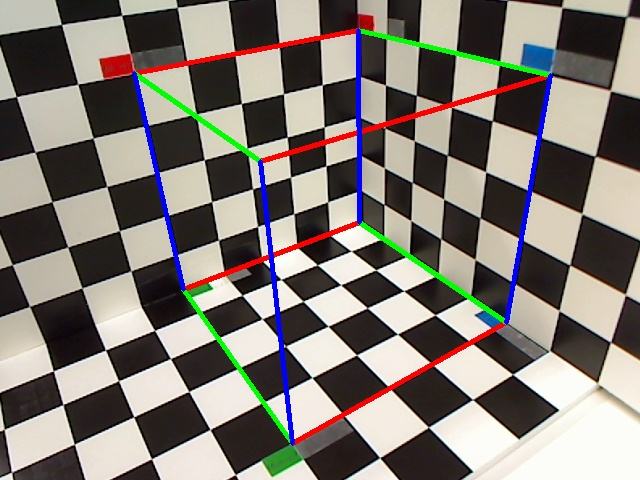
\includegraphics[height=60mm,bb=0 0 640 480]{image/task0.jpg}
  \figcaption{サンプル画像への立方体の描写}
  \label{fig:サンプル画像への立方体の描写の写真}
\end{figure}


\subsection{画像の射影行列の推測}
\label{sub:result_syaei}

別方向から撮影した 2 枚の画像についてキャリプレーションした結果を図\ref{fig:input0}、図\ref{fig:input1}に示した。
推定した射影行列による 2 次元座標と 3 次元座標上の点はほぼ一致していることがわかる。

\begin{figure}[H]
  \centering
  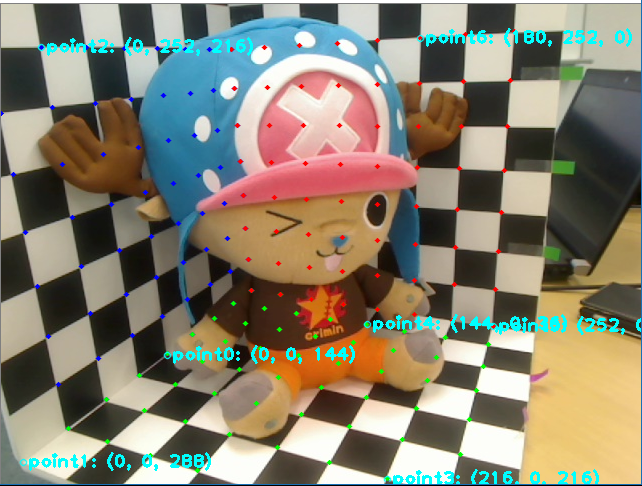
\includegraphics[height=50mm,bb=0 0 642 486]{image/input0.png}
  \figcaption{画像の射影行列の推測(1)}
  \label{fig:input0}
\end{figure}

\begin{figure}[H]
  \centering
  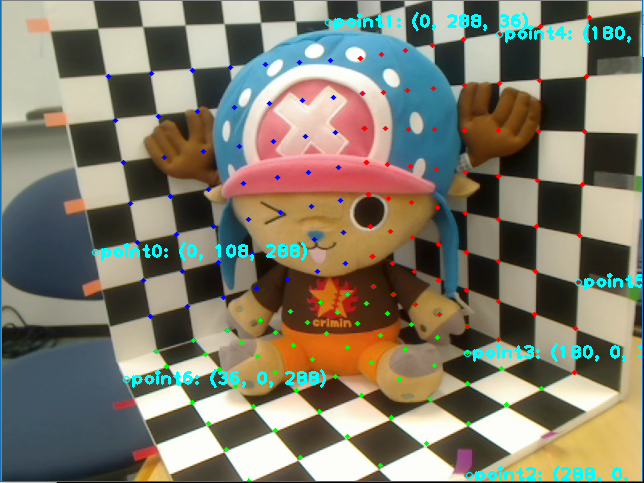
\includegraphics[height=50mm,bb=0 0 644 483]{image/input1.png}
  \figcaption{画像の射影行列の推測(2)}
  \label{fig:input1}
\end{figure}


\subsection{多視点画像からの立体形状の復元}
\label{sub:result_multimage}

立体形状の復元を行ったのちに、前から見える様子をCGで再現してみた
その結果が図\ref{fig:capture}である。

\begin{figure}[H]
  \centering
  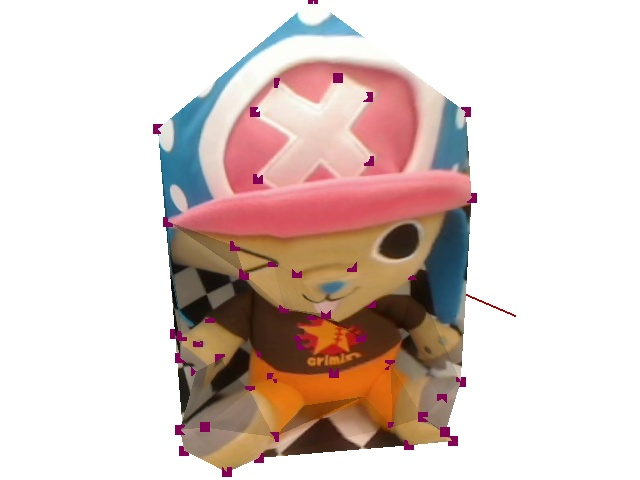
\includegraphics[height=50mm,bb=0 0 644 483]{image/task2.jpg}
  \figcaption{多視点画像から復元した立体形状の正面からのCG}
  \label{fig:capture}
\end{figure}



\subsection{立体形状からアナグリフの作成}
\label{sub:result_anaglyph}

CG描画した形状をアナグラフ表示した結果を図\ref{fig:anaglyph}に示した。


\begin{figure}[H]
  \centering
  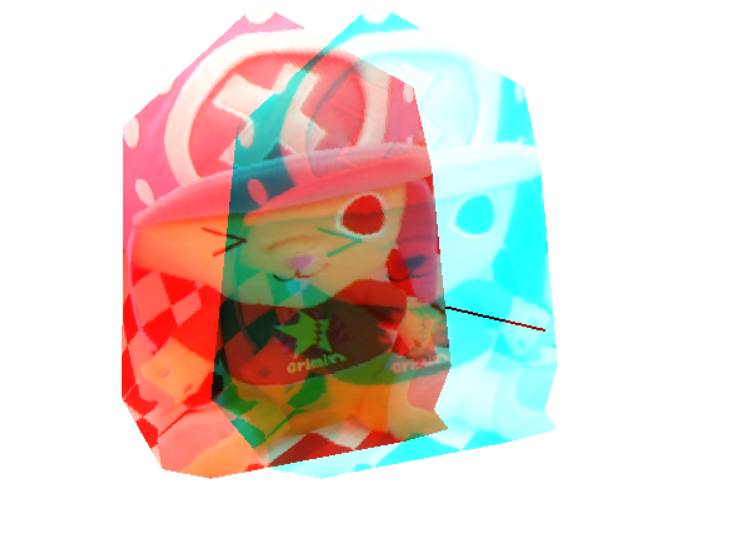
\includegraphics[height=60mm,bb=0 0 735 535]{image/ana.png}
  \figcaption{アナグリフ画像}
  \label{fig:anaglyph}
\end{figure}


\section{考察}
\label{sec:考察}

\subsection{画像から推測した射影行列の誤差}
\label{sub:画像から推測した射影行列の誤差}

まずは、絶対に発生しているであろう誤差として、クリックしたときに画像上で正確な点をクリックできていないというものである。
これを回避するためには、拡大してより誤差が小さくなるようにしてクリックするなどが考えられる。

そして他にも、手でクリックするのではなく、プログラム的に特徴点を検出して調べるという方法が考えられる。
今回の実験においては、背景にはチェックボートをおいているため、白と黒を検出するプログラムを
作ることができればより誤差は小さくすることができるであろう。

また、他にもカメラの解像度を上げたり、近づいた写真をとることで、誤差を減らすことができると思われる。
ただし、この方法では、カメラの性能が要求されたり、全体をキャプチャするのが大変であったりと、欠点もある。

ここで改めて、実際に生じる誤差について考えてみる。
今回キャプチャに用いた入力の画像は$640 \times 480$の画像であった。
カメラの中心軸で、$10\mathrm{cm}$離れた場所での写真に写る範囲が$32\mathrm{cm} \times 24\mathrm{cm}$
だったとする。そうすると、この距離にあるものをポイントしたとき1画素のずれがあったとすると、
実際の距離としては、0.5mmとなる。
正確に測っていたわけではないので、データの有意性はあまりありませんが、30cmほど離れた位置から写真を
撮って、そこでの写っている範囲は、おおよそ$64\mathrm{cm} \times 48\mathrm{cm}$ほどであったように思われる。

もしそうであったとすると、誤差としては、1画素あたり1mmほどでないかと考えられる。

\subsection{物体全体をキャプチャする方法について}
\label{sub:物体全体をキャプチャする方法について}

2枚だけでは画像の影になった部分について画像を得ることができず、立体形状を取得できない。
つまり、画像の影になった部分について立体形状を取得できない欠点がある。
これを解決するためには、より多くの画像からテスクチャと位置情報を得ればよいであろう。
そのときには、手でクリックするのではなく、もっとより正確でよりより方法が必要となると思われる。

そのときの方法としては、同じ視点から撮った画像において、マーカーをつけたと写真と、マーカーをつけていない
二枚を撮っておいて、マーカー付きの写真はクリックするために用いて、マーカーをつけていないものを
テクスチャとして用いる方法が考えられる。

また、写真の共通点を認識する技術としては、SIFTという特徴点を検出する方式によって行うという方法も
あるということがわかった。

\subsection{SIFTについて}
\label{sub:SIFTについて}

\ref{sub:物体全体をキャプチャする方法について}節で少し触れたSIFTについて、興味を持ったため
少し調べて考察を加えてみる。
SIFTとは特徴的な場所を見つけるというものである。

大まかな流れとしては、特徴点を見つけて、その特徴量を記述するとなる。
優れている点としては、スケールや回転、照明の強度に対して頑健な特徴量となっているところである。
今回の実験にもし用いることができたならば、大変精度の高い立体形状の復元ができたのではないかと思う。


SIFTを使ったアプリケーションとしては、私たちが一番よく使うところでは、
パノラマ写真の合成などに用いられている。
大きさや回転に対して強いという特徴があるため、他にも多くの応用方法がある。
例えば、物体認識や画像分類などといったことである。

\subsection{三角メッシュについて}
\label{sub:三角メッシュについて}
\ref{sub:多視点画像からの立体形状の復元}節では、三点以上クリックされると、三角のメッシュを
生成しながら、立体形状の復元を行っていった。このときの三角メッシュの作成は
``ドロネーの三角形分割''というアルゴリズムに沿って分割が行われていることがわかる。
このアルゴリズムについて調べてみた。

アルゴリズムは何通りかあるが、ここでは一番シンプルなものを取り上げる。

今回は点をどんどんとクリックしていき、徐々に三角形でメッシュする範囲が広がっていくので
``逐次添加法''と呼ばれるアルゴリズムが一番わかりやすいかと思う。

そのアルゴリズムとは、
\begin{itemize}
  \item まずは、画像内に3点入れたときをスタートする。ここから3角形が作られる。
  \item つぎに、点をどこかに追加することになる。
  \begin{itemize}
    \item この点が、すでにできている三角メッシュの中に含まれない場合は
    その点から最も近い2点を選んんでその点に対して辺を作成して新たな三角形を作成する。
    \item この点が、三角メッシュの中のある三角形の辺上であった場合は
    その辺の対角線上にある点と、追加した点を結んで、新たな辺として三角形を作る。
    \item この点が、ある三角形の中にあった場合は、その三角形の頂点に対して新たに3本の線を引いて
    辺とすることで、三角形を作る。
  \end{itemize}
  \item 点を追加した後に新しくできた辺に対して、ドロネーの三角分割法おいて不正な辺である可能性があるので
  それを確かめる。
\end{itemize}

不正な辺について
\begin{itemize}
  \item ドロネーの三角分割法においては、ある辺をとりだして、それを含む、二つの三角形の辺上にない
  二つの頂点を取り出す。これをA,Bとする。
  \item Aと辺を含む三角形の外接円のなかにBが入っていた場合、それは不正な辺であり、フリップを行う。
  \item その逆も確かめる。不正であればフリップを行う。
  \item フリップの操作としては、取り上げた辺を消して、A,Bに新しい辺を作ることである。
\end{itemize}

なぜ、このような操作を行うのかというと、高さ(または深さ)を正確に測るという目的がある。

例えば、とある連なった山に対して、尾根に点をおいたとする。
(図\ref{fig:delaunay}を参考)
※\cite{kimura}より画像を引用させていただいた

最初に尾根上に辺を作ることができればだいたい正しい値の高さが得ることができるが、
このとき、尾根上でない、斜面に向かって辺を引いてしまった場合、高さが低くなってしまう。
このようなことを避けることができるためドロネーの三角形分割法は用いられる。

\begin{figure}[H]
  \centering
  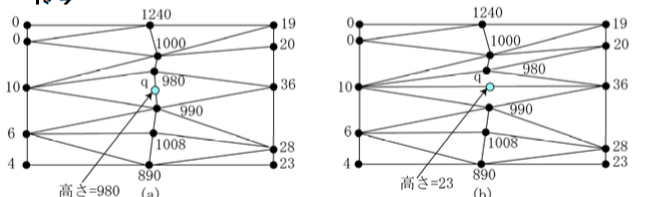
\includegraphics[height=30mm,bb=0 0 657 197]{image/delaunay.png}
  \figcaption{ドロネーの三角分割法について}
  \label{fig:delaunay}
\end{figure}

\section{結論と感想}
\label{sec:結論と感想}
射影行列により、3次元の座標から、2次元の座標への変換が可能、
何個かの2次元座標と、3次元座標の組み合わせで射影行列の推定が可能、
多視点画像とその画像の射影行列が分かれば、立体形状が復元可能である。

実験を通して、CGに対する理解が深まって大変良かったです。
SIFTやドロネー三角分割などといった、新しいアルゴリズムにも触れることができて面白かったです。
本実験が5個目の実験ですが、一番興味を持って望むことができました。

最近、自分の写真をグーグルフォトにバックアップしているのですが、たまに自動でパノラマ写真を合成して
通知してくれることがあり、そのなかではこのような画像処理が行われているのだろうかと思うと
なんだかわくわくしますね。

今回のレポートではSIFTのアルゴリズムは理解しきれなかったので、あらためて時間を割いて
理解していきたいなと思います。


\begin{thebibliography}{9} %ケタ数(9:一桁、99:二桁)
\bibitem{saito} 斎藤英雄 , ``画像からの立体形状キャプチャ'' , 2016
\bibitem{sift1} 中央大学 藤吉研究室 , ``画像局所特徴量と特定物体認識'' ,\url{http://www.vision.cs.chubu.ac.jp/cvtutorial/PDF/02SIFTandMore.pdf} , アクセス日時 2016/06/30
\bibitem{sift2} 東京工業大学 長橋研究室 , ``SIFT画像処理'' ,\url{http://www.isl.titech.ac.jp/~nagahashilab/member/longb/iip/LectureNotes/sift_image.pdf} , アクセス日時 2016/06/30
\bibitem{sift3} ``画像処理を始めよう ー特徴量2 SIFTー'' ,\url{http://nodamushi.hatenablog.com/entry/20131208/1386475091} , アクセス日時 2016/06/30
\bibitem{sift4} lawmn ,``画像認識の初歩、SIFT,SURF特徴量'' ,\url{http://www.slideshare.net/lawmn/siftsurf} , アクセス日時 2016/06/30
\bibitem{aizu} 会津大学 , ``ドローネ三角形分割法'' , \url{http://i-health.u-aizu.ac.jp/CompuGeo/2013/handouts/chapter5/Chapter5H.pdf} , アクセス日時 2016/06/30
\bibitem{kimura} 木村 元 ,``計算幾何学と関数近似 自己組織化'' ,\url{http://sysplan.nams.kyushu-u.ac.jp/gen/edu/SystemsDesign/2008/kougi09/kougi09.pdf} ,アクセス日時 2016/06/30
\bibitem{taseru} たーせる , ``ProcessingでDelaunay分割(解説篇)'' , \url{http://tercel-sakuragaoka.blogspot.jp/2011/06/processingdelaunay_3958.html} ,アクセス日時 2016/06/30
\end{thebibliography}

\end{document}
